\documentclass[11pt, a4paper]{article}

\usepackage[utf8]{inputenc}
\usepackage{graphicx}
\graphicspath{ {images/} }
\usepackage{mathtools}
\usepackage{amssymb}
\usepackage{amsmath}
\usepackage[ngerman,english]{babel}
\usepackage{cite}
\usepackage{bibgerm}
\usepackage{fullpage}
\usepackage[top=1.5cm,bottom=1.5cm,left=3.5cm,right=2.5cm,headsep=1.5cm,includeheadfoot]{geometry}
\usepackage{tabularx}
\usepackage{caption}
\usepackage{subcaption}
\usepackage{eurosym}
\usepackage{enumitem}
\usepackage{multicol}
\usepackage{tikz}
\usepackage{tkz-euclide}
\usepackage{pgfplots}
\usepackage{pdflscape}
\usepackage{acronym}
\usepackage{blindtext}
\usepackage{ifthen}
\usepackage{setspace}
\usepackage{cancel}
\usepackage{color}
\usepackage{listings}
\usepackage{comment}
\usepackage{xcolor}
\usepackage{colortbl}
\usepackage[parfill]{parskip}
\usepackage{url}

\usepackage{fancyhdr}
\pagestyle{fancy}

\fancyhf{} % clear all
\fancyhead[L]{\leftmark}
\fancyfoot[C]{-- \thepage{} --}
%\setlength{\headheight}{15pt}
\renewcommand{\headrulewidth}{0.5pt}
\renewcommand{\footrulewidth}{0pt}
\setlength{\skip\footins}{0.7cm}

\usetikzlibrary{graphs}
\usetikzlibrary{positioning}

\onehalfspacing
\setlength\parindent{0pt}

%\everymath{\displaystyle}

\allowdisplaybreaks

\definecolor{AI-BLUE}{rgb}{0,0.57,0.87}

% Eigene Befehle
\newcommand\q[1]{\emph{"#1"}}
\renewcommand\equiv{\Leftrightarrow}
\newcommand\vertequal[2]{\underset{\underset{#2}{\parallel}}{#1}}
\newcommand\cif{\text{if }}
\newcommand\abs[1]{\left|#1\right|}
\newcommand\norm[1]{\abs{\abs{#1}}}
\newcommand\diff[1]{\text{ d#1}}
\newcommand\av[1]{\left\langle#1\right\rangle}
\newcommand\ev[1]{\mathbb{E}\left(#1\right)}
\newcommand\br[1]{\left(#1\right)}
\newcommand\ubr[2]{\underbrace{#1}_{#2}}
\newcommand\quer[1]{\overline{#1}}
\newcommand\setequal{\overset{!}{=}}
\newcommand\dint{\displaystyle \int}
\newcommand\dsum{\displaystyle \sum}
\newcommand\dprod{\displaystyle \prod}
\newcommand\closedInt[2]{\left[#1,#2\right]}
\newcommand{\checkbox}{\Large \Square \normalsize \hspace{0.4cm}}

\newcommand\V[1]{\ensuremath{\underline{\mathbf{#1}}}}
\newcommand\M[1]{\ensuremath{\underline{\underline{\mathbf{#1}}}}}

\newcommand\myref[1]{\ref{#1} (S. \pageref{#1})}
\newcommand\myrefcomma[1]{\ref{#1}, S. \pageref{#1}}

\begin{document}

\thispagestyle{empty}

\setlength{\hoffset}{-0.5cm} % center title page

\lstset{
  basicstyle=\small,           % the size of the fonts that are used for the code
  breaklines=true,             % sets automatic line breaking
  captionpos=b,                % sets the caption-position to bottom
  frame=single,                % adds a frame around the code
  keepspaces=true,             % keeps spaces in text, useful for keeping indentation of code (possibly needs columns=flexible)
  numbers=right,               % where to put the line-numbers; possible values are (none, left, right)
  showspaces=false,            % show spaces everywhere adding particular underscores; it overrides 'showstringspaces'
  stepnumber=1,                % the step between two line-numbers. If it's 1, each line will be numbered
  tabsize=4,                   % sets default tabsize to 4 spaces
  xleftmargin=0.14cm		   % sets left margin
}

\begin{titlepage}
    \begin{center}
    \Large \textbf{Master's Thesis}\\
    \vspace{3cm}
    \normalsize
    Master's Thesis\\
    in the Program of Applied Computer Science\\
    at the Ruhr-University Bochum\\
    at the Institute for Neural Computation\\
    in the Summer Term 2016\\
    \vspace{3cm}
    \LARGE \textbf{A Deep Convolutional Network for Facial Landmark Estimation} \\
    \vspace{3cm}
    \normalsize
    \textbf{Author:}\\
    Schrör, Phil Yannick\\
    108 011 214 024\\
    \vspace{2cm}
    \textbf{To be handed in:}\\
    31st of October 2016\\
    \vspace{2cm}
    \textbf{Supervisors:}\\
    PD Dr. Rolf P. Würtz\\
    M.Sc. Andreas Nilkens
    \end{center}
\end{titlepage}

\newpage
\pagenumbering{Roman}
\setcounter{page}{2}

\tableofcontents

\newpage

\addcontentsline{toc}{section}{List of Acronyms}

\section*{List of Acronyms}
\markboth{LIST OF ACRONYMS}{}

%\acrodefplural{KNN}[KNN]{Künstliche Neuronale Netzwerke}

\begin{acronym}
\acro{ANN}{Artificial Neural Network}
\acro{CNN}{Convolutional Neural Network}
\acro{MSSE}{Mean Summed Squared Error}
\acro{MUCT}{Milborrow / University of Cape Town} (Image data set)
\acro{ReLU}{Rectified Linear Unit}
\acro{RGB}{Red Green Blue}
\acro{RNN}{Recurrent Neural Network}
\acro{SGD}{Stochastic Gradient Descent}
\end{acronym}


%\subsection*{Color legend} %TODO Remove me
%\textcolor{purple}{purple: find better synonym}

\newpage

\setcounter{page}{1}
\pagenumbering{arabic}

%%%%%%%%%%%%%%%%%%%%%%%%%%%%%%%%%%%%%%%%%%%%%%%%%%%%%%%%%%%%%%%%%%%%%%%%%%%%%%%%%%%%%%%%%%%%%%%%%%%%%%%%%
%%%%%%%%%%%%%%%%%%%%%%%%%%%%%%%%%%%%%%%%%%%%%%%%%%%%%%%%%%%%%%%%%%%%%%%%%%%%%%%%%%%%%%%%%%%%%%%%%%%%%%%%%
%									INTRODUCTION CHAPTER BEGINS HERE									%
%%%%%%%%%%%%%%%%%%%%%%%%%%%%%%%%%%%%%%%%%%%%%%%%%%%%%%%%%%%%%%%%%%%%%%%%%%%%%%%%%%%%%%%%%%%%%%%%%%%%%%%%%
%%%%%%%%%%%%%%%%%%%%%%%%%%%%%%%%%%%%%%%%%%%%%%%%%%%%%%%%%%%%%%%%%%%%%%%%%%%%%%%%%%%%%%%%%%%%%%%%%%%%%%%%%

\section{Introduction}

\acp{ANN} have proven to be very powerful tools developed and used in the field of Neural Computation. Particularly \acp{CNN} exhibit a solid performance on graphical data like images or videos. Finding patterns and hidden structures in images can be very useful in many respects, one of them the diagnosis of diseases which influence the appearance of the human face\footnote{cf. \cite{ebgm}}. For that reason \acp{CNN} are used in the scope of this thesis to estimate the position of so called landmarks in images of human faces. While some of those landmarks are preeminent features like the eyes or the tip of the nose, other landmarks are less prominent points, which are harder to find.\\
Since tagging all those landmarks by hand is a tedious work, it is desirable to create an automatism, which estimates them. In order to reach this goal two different general network architectures are used and tested in many different configurations. Both kinds of network take an RGB-image of a human face as input and produce the estimated coordinates of the landmarks as output. The first approach, however, trains a complete \ac{CNN} conventionally, i.e. all the network's weights are initialized randomly and subsequently trained by the \ac{SGD} optimization method. The second approach, on the other hand, uses Gabor wavelets as weights for the first layer of the \ac{CNN}. In this kind of network only the weights of the subsequent layers are trained, while the Gabor wavelets remain unchanged throughout the whole training process. The Gabor responses are then combined and forwarded through the subsequent layers of the network.\\
In order to compare the two approaches a \ac{CNN} with the same structure as used with the Gabor wavelets has been trained completely. \dots\\%TODO Elaborate this
Testing the different networks has shown that \dots%TODO Write more!
% Completely trained network with the dimensions of the gabor network
% Hint some of the results
% Explain how this thesis is organized

\newpage

%%%%%%%%%%%%%%%%%%%%%%%%%%%%%%%%%%%%%%%%%%%%%%%%%%%%%%%%%%%%%%%%%%%%%%%%%%%%%%%%%%%%%%%%%%%%%%%%%%%%%%%%%
%%%%%%%%%%%%%%%%%%%%%%%%%%%%%%%%%%%%%%%%%%%%%%%%%%%%%%%%%%%%%%%%%%%%%%%%%%%%%%%%%%%%%%%%%%%%%%%%%%%%%%%%%
%							ARTIFICIAL NEURAL NETWORKS CHAPTER BEGINS HERE								%
%%%%%%%%%%%%%%%%%%%%%%%%%%%%%%%%%%%%%%%%%%%%%%%%%%%%%%%%%%%%%%%%%%%%%%%%%%%%%%%%%%%%%%%%%%%%%%%%%%%%%%%%%
%%%%%%%%%%%%%%%%%%%%%%%%%%%%%%%%%%%%%%%%%%%%%%%%%%%%%%%%%%%%%%%%%%%%%%%%%%%%%%%%%%%%%%%%%%%%%%%%%%%%%%%%%

\section{Artificial Neural Networks}

\acp{ANN} are one of the most common models of Machine Learning or more specifically of Supervised Learning. They are basically mathematical functions, which take an input vector \V{x} and map it to an output vector \V{y}. They are usually constructed as an ensemble of several layers, which for their part consist of many individual units which are called neurons. \acp{ANN} have a huge span of applications and can be used for classification and regression tasks, e.g. predicting the class of a traffic sign from an image (classification) or estimating the weight of a person depicted on a photo (regression). \acp{ANN} have proven to be very powerful, in fact, the Universal Approximation Theorem states that \q{there is a single hidden layer feed-forward network that approximates any measurable function to any desired degree of accuracy on some compact set K [...]}\footnote{cf. \cite{uat}, p. 4, corollary 2.1}. Hence, there exists a suitable neural network for almost any practical application. The remaining problem is that there is no guarantee for the existence of a learning algorithm, which is able to find the necessary network parameters. Nonetheless, there are many problems on which \acp{ANN} perform very well.

\subsection{Artificial Neurons}

Natural neurons are the information transmitting and processing units of the brain of animate beings such as the human. While there are various types of natural neurons, which function in different ways, artificial neurons as their mathematical counterpart are reduced to the basic functionality. Natural neurons receive and send signals from and to other neurons via synapses. A synapse is a link between the spike emitting axon of the pre-synaptic neuron and the spike receiving dendrites or soma of the post-synaptic neuron. Each synapse has a certain strength, according to which it increases or decreases the post-synaptic neuron's activation, depending on whether it is an excitatory synapse or an inhibitory synapse. Figure \ref{fig:two_connected_neurons} illustrates two connected neurons:

\begin{figure}[htbp]
\centering
	\begin{tikzpicture}[xscale=1.2, every path/.style={>=latex}]
	\node (N1) at (0,0) [circle,draw,minimum size=1cm] {N1};
	\node [below=0.05cm of N1]{Soma};
	\node (Synapse) at (2,0) [rectangle,draw] {\hspace{0.2cm}};
	\node [below=0.1cm of Synapse]{Synapse};
	\node (N2) at (4,0) [circle,draw,minimum size=1cm] {N2};
	\node [below=0.05cm of N2]{Soma};
	\draw[->] (N1) to node[above]{Axon} (Synapse);
	\draw[->] (N2) to node[above]{Axon} (5.9,0);
	\draw[->] (-2,0.) to node[above]{Dendrite} (N1);
	\draw[->] (Synapse) to node[above]{Dendrite} (N2);
	\end{tikzpicture}
\caption{Two connected neurons N1 and N2}
\label{fig:two_connected_neurons}
\end{figure}
\vspace{-0.2cm}
In artificial neurons complicated electrical or chemical transmitting mechanisms consisting of the axon of the spiking neuron, the dendrite or soma of the receiving neuron and the synapse and its strength in between are replaced by a single number, the so called weight, which determines the strength of the synapse. If it is positive, the synapse or connection is excitatory, otherwise it is inhibitory. Figure \ref{fig:two_neurons_weight} shows two connected artificial neurons.

\begin{figure}[htbp]
\centering
	\begin{tikzpicture}[xscale=1.2, every path/.style={>=latex}]
	\node (N1) at (0,0) [circle,draw,minimum size=1cm] {N1};
	\node (N2) at (3,0) [circle,draw,minimum size=1cm] {N2};
	\draw[->] (N2) to (4.9,0);
	\draw[->] (-2,0.) to (N1);
	\draw[->] (N1) to node[above]{weight} (N2);
	\end{tikzpicture}
\caption{The complicated natural neurons' mechanisms are replaced by a weight}
\label{fig:two_neurons_weight}
\end{figure}

 Unlike natural neurons, which receive spikes and fire (emit a spike) at discrete points in time, the membrane potential or activation of artificial neurons is averaged over time and represented by a single scalar value for simplicity reasons. The averaging of time allows for a time-independent mathematical function, whose value can be calculated without looking at each neuron at numerous points in time to find out its current activation. Formula \eqref{eq:mathematical_neuron} shows how the mathematical formula of an artificial neuron looks like so far:
\begin{align}
\label{eq:mathematical_neuron}
a_i = \sum_j w_{ij} \cdot a_j
\end{align}
Firstly, the activation $a_j$ of each preceding neuron $j$ is multiplied with the weight of the synapse from neuron $j$ to neuron $i$. All these products add up to the activation $a_i$ of neuron $i$. Until now artificial neurons are linear units. Combining them yields a completely linear function. Hence, there is no real advantage in combining many neurons into a whole network, because it would not be more powerful than a single neuron. Speaking about classification, such a network still divides the space of all possible inputs linearly, which leads to bad results if the input data is not linearly separable. The true power of \acp{ANN} originates from their non-linearity, which is induced by so called activation functions.

\subsection{Activation Functions}

Natural neurons collect spikes over time and accumulate them. Each time, when a spike arrives at the neuron, the membrane potential increases. Over time the potential decreases, but if sufficiently many spikes reach the neuron before its membrane potential has decreased too much, a spike is emitted. This biological concept is transfered to the artificial neurons by means of activation functions. Before the membrane potential of a neuron is propagated forward to other neurons, an activation function is applied to it. However, all time related aspects are neglected in classical \acp{ANN}. Only more sophisticated neural networks like Spiking Neural Networks try to emulate the operation mode of time dependent natural neurons.\\
The most well-known activation function is probably the sigmoid (or sigmoidal) function, which is illustrated in figure \ref{fig:sigmoid} and whose standard formula is given in equation \eqref{eq:sigmoid}.
\begin{align}
\label{eq:sigmoid}
\sigma(a) = \frac{1}{1 + e^{-a}}
\end{align}

\begin{figure}[htbp]
	\centering
	\begin{tikzpicture}[yscale=1.9,xscale=1.25]
		\def \xMin {-4};
		\def \xMax {4};
		\def \yMin {0};
		\def \yMax {1.};
		\draw[->] (\xMin - 0.3,0) -- (\xMax + 0.3,0) node[right] {$a$};
		\draw[->] (0,\yMin - 0.3) --(0,\yMax + 0.3) node[above] {$\sigma(a)$};
		\draw[domain=\xMin:\xMax,samples=30,variable=\x,blue]
			plot ({\x},{1 / (1 +  exp(-\x))});
		\foreach \tic in {\yMin,...,\yMax}
     	{
     		\draw[shift={(0,\tic)},color=black] (3pt,0pt) -- (-3pt,0pt) node[left] {$\tic$};
     	}
     	\foreach \tic in {\xMin,...,\xMax}
     	{
     		\draw[shift={(\tic,0)},color=black] (0pt,3pt) -- (0pt,-3pt) node[below] {$\tic$};
     	}
 
	\end{tikzpicture}
	\caption{Sigmoid activation function}
	\label{fig:sigmoid}
\end{figure}

If the membrane potential $a$ is large, $e^{-a}$ tends to zero, so the output of the activation function $\sigma(a)$ is close to 1. If $a$ is very far in the negative area, $e^{-a}$ tends to $+\infty$ and thus $\sigma(a)$ is almost $0$. Summarized, a high (positive) membrane potential leads to a large output and a negative membrane potential leads to nearly no output. To individualize the activation function to a specific task, the formula can be extended so that the activation function becomes steeper. Formula \eqref{eg:steeper_sigmoid} shows the extended form:
\begin{align}
\label{eg:steeper_sigmoid}
\sigma(a) = \frac{1}{1 + e^{-\beta (a - a_0)}}
\end{align}

The parameter $\beta$ can be used to make the function steeper or less steep. $u_0$, however, can be used to shift the activation function to the left or to the right. Figure \ref{fig:modified_sigmoid} shows the sigmoid function with two different values for $\beta$:

\begin{figure}[htbp]
	\centering
	\begin{tikzpicture}[yscale=1.9,xscale=1.25]
		\def \xMin {-5};
		\def \xMax {5};
		\def \yMin {0};
		\def \yMax {1.};
		\draw[->] (\xMin - 0.3,0) -- (\xMax + 0.3,0) node[right] {$a$};
		\draw[->] (0,\yMin - 0.3) --(0,\yMax + 0.3) node[above] {$\sigma(a)$};
		\draw[domain=\xMin:\xMax,samples=30,variable=\x,blue]
			plot ({\x},{1 / (1 +  exp(-1.9*\x))}) node[above] {$\beta=1.9$};
		\draw[domain=\xMin:\xMax,samples=30,variable=\x,red]
			plot ({\x},{1 / (1 +  exp(-0.7*\x))}) node[below] {$\beta=0.7$};
		\foreach \tic in {\yMin,...,\yMax}
     	{
     		\draw[shift={(0,\tic)},color=black] (3pt,0pt) -- (-3pt,0pt) node[left] {$\tic$};
     	}
     	\foreach \tic in {\xMin,...,\xMax}
     	{
     		\draw[shift={(\tic,0)},color=black] (0pt,3pt) -- (0pt,-3pt) node[below] {$\tic$};
     	}
 
	\end{tikzpicture}
	\caption{Two variations of the sigmoid activation function}
	\label{fig:modified_sigmoid}
\end{figure}

Another variant of the sigmoidal function is the hyperbolic tangent $\tanh(a)$, which is equivalent to the sigmoidal function except for some linear transformations.
Including the activation function in our model, the formula for an artificial neuron changes as shown in equation \eqref{eq:mathematical_neuron_with_sigmoid}.
\begin{align}
\label{eq:mathematical_neuron_with_sigmoid}
a_i = \sum_j w_{ij} \cdot \sigma(a_j)
\end{align}
By adding the activation function, the model becomes non-linear. A sufficiently large \ac{ANN}, which connects many neurons to a whole network, is able to produce very sophisticated decision functions. Even if the sigmoidal activation function often works very well and has been analyzed very keenly, its rather high computation cost due to the exponential function is a clear disadvantage. Hence, less costly functions like the \ac{ReLU} have been developed. Its formula is given in equation \eqref{eq:relu}.

\begin{align}
\label{eq:relu}
\operatorname{ReLU}(a) = \begin{cases}a, \text{ if } a > 0\\0, \text{ else}\end{cases}
\end{align}

Figure \ref{fig:relu} shows the plot of this activation function:

\begin{figure}[htbp]
	\centering
	\begin{tikzpicture}[scale=0.85]
		\def \xMin {-4};
		\def \xMax {4};
		\def \yMin {-0.};
		\def \yMax {4.};
		\draw[->] (\xMin - 0.3,0) -- (\xMax + 0.3,0) node[right] {$a$};
		\draw[->] (0,\yMin - 0.3) --(0,\yMax + 0.3) node[above] {$\operatorname{ReLU}(a)$};
		\draw[domain=0:\xMax,samples=30,variable=\x,blue] plot ({\x},{\x});
		\draw[domain=\xMin:0,samples=2,variable=\x,blue] plot ({\x},{0});
		\foreach \tic in {\yMin,...,\yMax}
     	{
     		\draw[shift={(0,\tic)},color=black] (3pt,0pt) -- (-3pt,0pt) node[left] {$\tic$};
     	}
     	\foreach \tic in {\xMin,...,\xMax}
     	{
     		\draw[shift={(\tic,0)},color=black] (0pt,3pt) -- (0pt,-3pt) node[below] {$\tic$};
     	}
 
	\end{tikzpicture}
	\caption{Rectified Linear Unit (ReLU)}
	\label{fig:relu}
\end{figure}

According to \cite{dsrnn}, the \ac{ReLU} is not only faster than the sigmoidal activation function and the hyperbolic tangent activation function, but also biologically more plausible. One reason for its plausibility is its linearity. Figure \ref{fig:biological_activation_function} shows an activation function, which is constructed on the basis of biological data. The area enclosed by the red rectangle resembles the shape of the \ac{ReLU} presented in figure \ref{fig:relu}.


\begin{figure}[htbp]
	\centering
	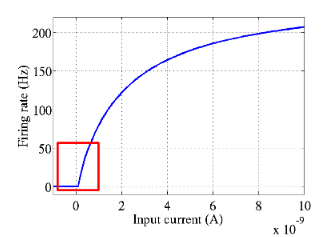
\includegraphics[width=0.6\textwidth]{biological_activation_function.png}
	\caption[Activation function inspired by biological data]{Activation function inspired by biological data\footnotemark}
	\label{fig:biological_activation_function}
\end{figure}
\footnotetext{Taken from \cite{dsrnn}, p. 3}


Another property of the \ac{ReLU}, which makes it biologically more plausible, is the fact that using the \ac{ReLU} as activation function leads to neural networks, which tend to be sparse. Sparse neural networks have only few connections or, equivalently, a lot of connections with a weight of zero. These networks are closer to natural neural networks, some of which appear to have only 1\% to 4\% of their neurons activated. On the one hand, sparse neural networks work well on naturally sparse data, on the other hand, a too sparse network may lose a lot of its modeling capability.\\
Being biologically plausible is not necessarily essential to construct a well performing machine learning model. However, in \cite{dsrnn} several comparisons between a network with the \ac{ReLU} as activation function and other models have shown that the \ac{ReLU} network performs better than the other models or is at least competitive. The \acp{CNN} used in this thesis often use combinations of the sigmoidal activation function and the \ac{ReLU}.

\subsection{Feed-forward Neural Networks}

The still most common \acp{ANN} are feed-forward neural networks. The neurons in a feed-forward neural network are usually organized in consecutive layers, which propagate the information in only one direction through the network. Figure \ref{fig:ffnn} shows a fully connected feed-forward network with one input layer, one output layer and two layers in between, which are called hidden layers.
\begin{figure}[htbp]
	\centering
	\begin{tikzpicture}[scale=1,every path/.style={>=latex}]
		%draw text nodes
		\node at (0,4.4) {Input Layer};
		\node at (9,4.9) {Output Layer};
		\node at (4.5,5.2) {Hidden Layers};
		% draw first layer
		\foreach \x in {1,...,3}
		{
			\node (n0\x) at (0, \x) [circle,draw,minimum size=0.5cm] {};
		}
		%draw second layer
		\foreach \x in {0,...,4}
     	{
     		\node (n3\x) at (3, \x) [circle,draw,minimum size=0.5cm] {};
     		% draw connections from layer one to layer two
     		\foreach \n in {1,...,3}
     		{
     			\draw[->] (n0\n) to (n3\x);
     		}
     	}
     	%draw third layer
		\foreach \x in {0,...,5}
     	{
     		\node (n6\x) at (6, \x - 0.5) [circle,draw,minimum size=0.5cm] {};
     		% draw connections from layer two to layer three
     		\foreach \n in {0,...,4}
     		{
     			\draw[->] (n3\n) to (n6\x);
     		}
     	}
     	%draw fourth layer
     	\foreach \x in {1,...,4}
     	{
     		\node (n9\x) at (9, \x - 0.5)  [circle,draw,minimum size=0.5cm] {};
     		% draw connections from layer three to layer four
     		\foreach \n in {0,...,5}
     		{
     			\draw[->] (n6\n) to (n9\x);
     		}
     	}
	\end{tikzpicture}
	\caption{Fully connected feed-forward neural network with two hidden layers}
	\label{fig:ffnn}
\end{figure}


As illustrated by the arrows in figure \ref{fig:ffnn}, the information is passed from the leftmost neurons in the input layer to the first hidden layer, then to the second hidden layer and finally to the output layer on the right. The number of neurons in the input layer has to correspond to the dimensionality of the input space. The number of neurons in the output layer is determined by the number of classes in a classification task or the number of desired outputs in a regression task respectively. Hence, these parameters are clearly defined by the problem and are not subject to the optimization process. On the other hand, the number of the neurons in the hidden layers and the number of the hidden layers itself depends on the complexity of the task, which shall be solved by the network. For easy solvable problems only a few neurons may suffice, while difficult tasks can require several hundred or thousand neurons. Figuring out an appropriate network architecture is a task, whose difficulty should be not underestimated.\\
The above depicted network is called fully-connected, because a neuron in layer $i$ has a connection to each neuron in layer $i + 1$. Note that there are no connections within one single layer. If there were also connections in the other direction, the network would be a \ac{RNN}. Although there are many interesting problems to which \acp{RNN} could be applied to, \acp{RNN} are much less prominent in Machine Learning, because there are very few well-established training algorithms. For feed-forward networks, however, exist reliable training algorithms. The most used of them is called Backpropagation. Backpropagation profits from the observation that a feed-forward \ac{ANN} is nothing more than a mathematical function, which fulfills the requirements for being differentiable. While the sigmoidal activation function and the hyperbolic tangent activation function are differentiable, the \ac{ReLU} is a bit problematic, because it is not differentiable at $0$. This problem can be eluded by setting the gradient to $0$ at this position. To understand how Backpropagation works, it is necessary to introduce an error function. The formula for a very common error function, the \ac{MSSE}, is given in equation \eqref{eq:msse}.
\begin{align}
\label{eq:msse}
\operatorname{MSSE} = \frac{1}{N} \cdot \sum_{i}^{N} \left(\hat{y}_i - y_i\right)^2
\end{align}
$N$ is the number of samples, e.g. the number of images used for training an \ac{ANN}. $\hat{y}_i$ is the predicted value for the $i$-th input vector $\V{x}_i$ and $y_i$ the true value, i.e. the label, of the said input. The goal of training an \ac{ANN} is to adapt its weights such that its prediction $\hat{y}_i$ is as close as possible to the true label $y_i$. In this case, the squared difference $(\hat{y}_i - y_i)^2$ is very small and does hardly contribute to the eventual value of the sum.\\
The value $\hat{y}_i$ is the result of the function, which is implemented by the neural network, and therefore depends mainly on the weights. Firstly, Backpropagation calculates the gradient of the error function with respect to the weights for a subset of the input data set by applying the chain rule. Since the gradient always points in the direction of the strongest increase, the weights are adapted by subtracting the gradient multiplied with a certain value, which is called learning rate. The learning rate determines how much influence the chosen subset of input data has on the weight changes. One way to chose the mentioned data subset is to consider all data and adapt the weights after presenting all inputs to the network, i.e. calculating the prediction $\hat{y}_i$ for each input vector $\V{x}_i$. The process of presenting all inputs is called an epoch. This method has the advantage of being relatively robust against noise, because it is averaged out to a certain degree. The disadvantage is that the weights are learned rather slowly, because a lot of epochs are needed until the network produces good results. Another way is to use small batches, i.e. the data is divided in $n$ equally sized subsets, which are subsequently presented to the network. Since the weights are adapted after each batch, the learning process should be faster. This method is called \acf{SGD}.\\
With $n_i$ as number of neurons in layer $i$, there are $n_i \cdot n_{i+1}$ connections between layer $i$ and layer $i+1$. That means that there are many connections, whose weights have to be learned during the training phase. Since the training time of such a network can easily last several days, more effective models are desirable.

\subsection{Convolutional Neural Networks}

\begin{itemize}
\item few weights
\item exploit 2D structure
\end{itemize}

\subsection{Deep Learning}

\begin{itemize}
\item many many many layers
\end{itemize\

\newpage

%%%%%%%%%%%%%%%%%%%%%%%%%%%%%%%%%%%%%%%%%%%%%%%%%%%%%%%%%%%%%%%%%%%%%%%%%%%%%%%%%%%%%%%%%%%%%%%%%%%%%%%%%
%%%%%%%%%%%%%%%%%%%%%%%%%%%%%%%%%%%%%%%%%%%%%%%%%%%%%%%%%%%%%%%%%%%%%%%%%%%%%%%%%%%%%%%%%%%%%%%%%%%%%%%%%
%									DATA CHAPTER BEGINS HERE											%
%%%%%%%%%%%%%%%%%%%%%%%%%%%%%%%%%%%%%%%%%%%%%%%%%%%%%%%%%%%%%%%%%%%%%%%%%%%%%%%%%%%%%%%%%%%%%%%%%%%%%%%%%
%%%%%%%%%%%%%%%%%%%%%%%%%%%%%%%%%%%%%%%%%%%%%%%%%%%%%%%%%%%%%%%%%%%%%%%%%%%%%%%%%%%%%%%%%%%%%%%%%%%%%%%%%

\section{Data}

Training and testing a \ac{CNN} requires an appropriate data set with a sufficiently large number of training and test examples. Daniel Nouri uses the data set from the \emph{Facial Keypoints Detection} challenge on the machine learning website Kaggle\footnote{cf. \cite{kaggle}} in his inspiring tutorial \emph{Using convolutional neural nets to detect facial keypoints}\footnote{cf. \cite{nouri-tutorial}}. This dataset provides a reasonable amount of landmarks, however, it does not provide all landmarks for all faces. To avoid too much data organization overhead it was used the \ac{MUCT} data set\footnote{cf. \cite{muct}} instead, which exhibits a simpler structure and provides not only all Kaggle landmarks but even more for each depicted person.

\subsection{Kaggle}

Since the first experiments done in the scope of this thesis were inspired by the tutorial by Daniel Nouri named above, it was initially worked with the same data set, which was used there. The contemplated data set is taken from the \emph{Facial Keypoints Detection} challenge on Kaggle and contains 7049 training images as well as 1783 test images with a resolution of $96 \times 96$ pixels. All images are provided as gray value images within the range $[0,255]$.\\
There are 15 different landmarks (called keypoints on Kaggle), each of which consists of two scalar values $(x,y)$, which represent the horizontal and vertical position of the corresponding feature in the image. The 15 landmarks are:
\begin{multicols}{2}
	\begin{itemize}[itemsep=-2ex]
		\item Left eye center
		\item Right eye center
		\item Left eye inner corner
		\item Left eye outer corner
		\item Right eye inner corner
		\item Right eye outer corner
		\item Left eyebrow inner end
		\item Left eyebrow outer end
	\end{itemize}
\columnbreak
	\begin{itemize}[itemsep=-2ex]
		\item Right eyebrow inner end
		\item Right eyebrow outer end
		\item Nose tip
		\item Mouth left corner
		\item Mouth right corner
		\item Mouth center top lip
		\item Mouth center bottom lip
	\end{itemize}
	\vphantom{}
\end{multicols}
%TODO Insert image which shows all the landmarks
As already mentioned, not all landmarks exist for all images. In fact, for almost all landmarks exists an individual number of images containing them. This leads to problems, because a \ac{CNN} expects a fixed number of inputs and a produces a fixed number of outputs. It is difficult to develop a mechanism, which checks for each input image how many landmarks are actually given and then includes only these landmarks into the calculation of the error function. Since using this data set would have required a comparatively high organization effort and since the resolution of $96 \times 96$ is rather small, another data set with a larger resolution of the raw images was used.

\subsection{MUCT Face Database}

The \acf{MUCT} face database was created by Stephen Milborrow, John Morkel and Fred Nicolls in December 2008 at the University Of Cape Town.\footnote{cf. \cite{muct}} It contains 3755 faces with 76 manually set landmarks, including all Kaggle landmarks presented above. As shown in figure \ref{fig:muctfaces}, it provides a broad spectrum of faces from people of different age, gender and ethnicity. Furthermore, many different lighting settings have been used in order to increase the diversity of the pictures.

\begin{figure}[htbp]
	\centering
	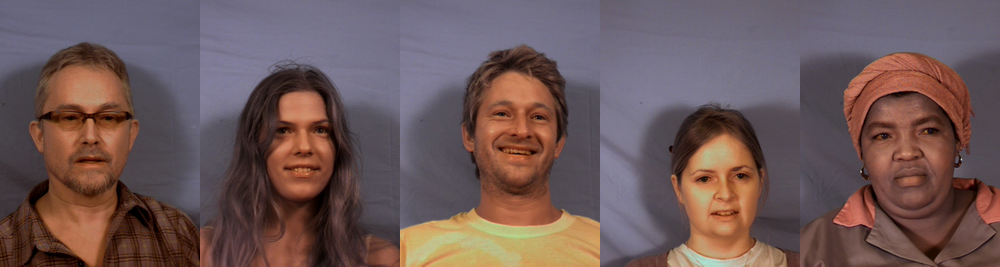
\includegraphics[width=\textwidth]{muct_faces.png}
	\caption{Five faces from the MUCT Face Database}
	\label{fig:muctfaces}
\end{figure}

Since images given in real applications are often not taken from a perfectly frontal perspective on the face, the creators of the data set provide images taken from five different angles, which are shown in figure \ref{fig:muctangles}. Disregarding some software induced delays, all five images were taken simultaneously in order to guarantee that the person does not move between two photo shots. Whereas two of the images show the right side of the person's face, images of the left side were not taken, because approximations of these images can be easily obtained by mirroring.

\begin{figure}[htbp]
	\centering
	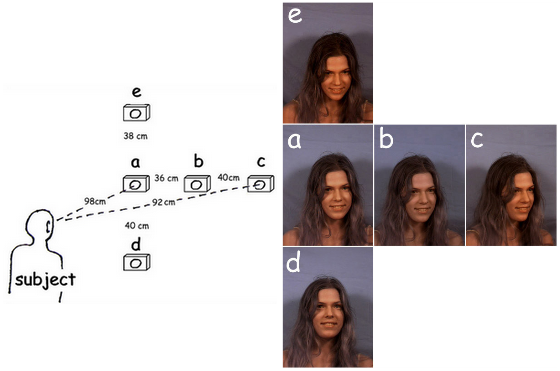
\includegraphics[width=0.77\textwidth]{muct_perspectives.png}
	\caption[MUCT Different Perspectives]{MUCT Different Perspectives\footnotemark}
	\label{fig:muctangles}
\end{figure}
\footnotetext{Both illustrations were taken from the \cite{muct} paper}

There is only one real disadvantage of the \ac{MUCT} data set compared to the Kaggle data set, i.e. the smaller total number of images -- 3755 on \ac{MUCT} instead of 8832 on Kaggle. Apart from that, using the \ac{MUCT} data set has a lot of advantages. The first one is the larger resolution: the \ac{MUCT} images are made available in a resolution of $480 \times 640$ pixels, whereas the Kaggle images have a resolution of only $96 \times 96$ pixels. Even if the full resolution cannot be used due to execution time and memory space restrictions, larger resolutions than $96 \times 96$ allow for a model, which works more precisely with regard to rather subtle or fine landmarks. Another advantage is the accessibility of color information, which may be useful to produce reasonable predictions at the expense of a longer program execution time.\\
Another expedient property of the \ac{MUCT} data set is its well-structuredness. The file names contain all relevant information about the corresponding image, because all of them follow the pattern: \texttt{i\{personID\}\{lighting set\}\{camera view\}-\{gender\}\{(no) glasses\}}. The first \texttt{i}mage of the data set has the file name \texttt{i000qa-fn.jpg}, so the person has the ID \texttt{000}, lighting setting \texttt{q} was used, the photo was shot from angle \texttt{a}, the person is \texttt{f}emale and does \texttt{n}ot wear glasses.\\
This naming system is highly valuable, because selecting only a certain subset of the images is simplified a lot, because it is sufficient to check their filename for a specific character at the position corresponding to the chosen criterion. This is important, because also the \ac{MUCT} data set does not provide all landmarks for all images, but it does so in a much more organized and transparent way. As pointed out in \cite{muct}, it occurs only for the camera views \texttt{b} and \texttt{c} that some landmarks may not be given, because some of them are not visible due to the perspective on the face. For example the ends of the persons' left eyebrows are often not visible.\\
Since \acp{ANN} usually require a fixed input size and a fixed output size, all images taken from camera view \texttt{b} and \texttt{c} were omitted and not used at all. For that reason the total number of images shrinks to 2257, which were divided randomly in 1752 training images and 502 test images by declaring 20\% of the persons as test persons. No person was assigned to both training set and test set in order to increase the generalization capability of the network. Hence, the test images presented to the network always showed persons unknown to the network.
%Maybe add something about the lighting settings, if there will remain too much unused space.

\subsection{Data Preprocessing}

\begin{itemize}
\item image size
\item auto contrast
\item normalization
\item gray scale
\end{itemize}

\newpage

%%%%%%%%%%%%%%%%%%%%%%%%%%%%%%%%%%%%%%%%%%%%%%%%%%%%%%%%%%%%%%%%%%%%%%%%%%%%%%%%%%%%%%%%%%%%%%%%%%%%%%%%%
%%%%%%%%%%%%%%%%%%%%%%%%%%%%%%%%%%%%%%%%%%%%%%%%%%%%%%%%%%%%%%%%%%%%%%%%%%%%%%%%%%%%%%%%%%%%%%%%%%%%%%%%%
%								NETWORK ARCHITECTURES CHAPTER BEGINS HERE								%
%%%%%%%%%%%%%%%%%%%%%%%%%%%%%%%%%%%%%%%%%%%%%%%%%%%%%%%%%%%%%%%%%%%%%%%%%%%%%%%%%%%%%%%%%%%%%%%%%%%%%%%%%
%%%%%%%%%%%%%%%%%%%%%%%%%%%%%%%%%%%%%%%%%%%%%%%%%%%%%%%%%%%%%%%%%%%%%%%%%%%%%%%%%%%%%%%%%%%%%%%%%%%%%%%%%

\section{Network Architectures}

\subsection{Initialization}

Cite Glorot! (again)

\subsection{Thoroughly trained CNN}

\subsection{Using Gabor Wavelets}

\subsubsection{Absolute value}
\subsubsection{Phase}
\subsubsection{Combining both approaches}

\newpage

%%%%%%%%%%%%%%%%%%%%%%%%%%%%%%%%%%%%%%%%%%%%%%%%%%%%%%%%%%%%%%%%%%%%%%%%%%%%%%%%%%%%%%%%%%%%%%%%%%%%%%%%%
%%%%%%%%%%%%%%%%%%%%%%%%%%%%%%%%%%%%%%%%%%%%%%%%%%%%%%%%%%%%%%%%%%%%%%%%%%%%%%%%%%%%%%%%%%%%%%%%%%%%%%%%%
%										RESULTS CHAPTER BEGINS HERE										%
%%%%%%%%%%%%%%%%%%%%%%%%%%%%%%%%%%%%%%%%%%%%%%%%%%%%%%%%%%%%%%%%%%%%%%%%%%%%%%%%%%%%%%%%%%%%%%%%%%%%%%%%%
%%%%%%%%%%%%%%%%%%%%%%%%%%%%%%%%%%%%%%%%%%%%%%%%%%%%%%%%%%%%%%%%%%%%%%%%%%%%%%%%%%%%%%%%%%%%%%%%%%%%%%%%%

\section{Results}

\subsection{Thoroughly trained CNN}

\begin{itemize}
\item Gridsearch
\item Momentum (bad!?)
\item Decay (bad, too!?)
\item Color vs no color
\end{itemize}

\subsection{Using Gabor Wavelets}

\begin{itemize}
\item Small resolution, absolute value
\item Small resolution, arctan2
\item Larger resolution, absolute value
\item Larger resolution, arctan2
\end{itemize}

\begin{figure}[htbp]
	\centering
	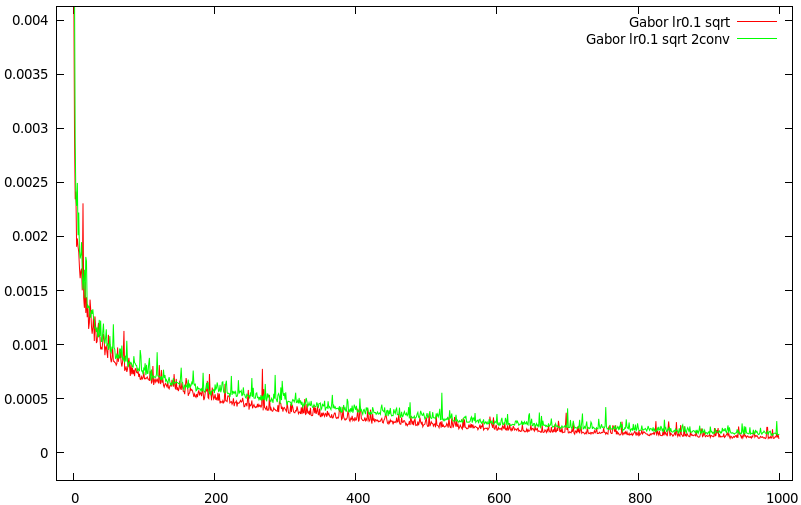
\includegraphics[width=\textwidth]{res_gabor_sqrt_vs_2conv.png}
	\caption{Results Gabor Sqrt vs 2Conv}
	\label{fig:res_gabor_sqrt_vs_2conv}
\end{figure}

\subsection{Confrontation of both Approaches}

Gabor approach probably better

\newpage

%%%%%%%%%%%%%%%%%%%%%%%%%%%%%%%%%%%%%%%%%%%%%%%%%%%%%%%%%%%%%%%%%%%%%%%%%%%%%%%%%%%%%%%%%%%%%%%%%%%%%%%%%
%%%%%%%%%%%%%%%%%%%%%%%%%%%%%%%%%%%%%%%%%%%%%%%%%%%%%%%%%%%%%%%%%%%%%%%%%%%%%%%%%%%%%%%%%%%%%%%%%%%%%%%%%
%									CONCLUSION CHAPTER BEGINS HERE										%
%%%%%%%%%%%%%%%%%%%%%%%%%%%%%%%%%%%%%%%%%%%%%%%%%%%%%%%%%%%%%%%%%%%%%%%%%%%%%%%%%%%%%%%%%%%%%%%%%%%%%%%%%
%%%%%%%%%%%%%%%%%%%%%%%%%%%%%%%%%%%%%%%%%%%%%%%%%%%%%%%%%%%%%%%%%%%%%%%%%%%%%%%%%%%%%%%%%%%%%%%%%%%%%%%%%

\section{Conclusion}

\newpage

%%%%%%%%%%%%%%%%%%%%%%%%%%%%%%%%%%%%%%%%%%%%%%%%%%%%%%%%%%%%%%%%%%%%%%%%%%%%%%%%%%%%%%%%%%%%%%%%%%%%%%%%%
%%%%%%%%%%%%%%%%%%%%%%%%%%%%%%%%%%%%%%%%%%%%%%%%%%%%%%%%%%%%%%%%%%%%%%%%%%%%%%%%%%%%%%%%%%%%%%%%%%%%%%%%%
%										APPENDIX BEGINS HERE											%
%%%%%%%%%%%%%%%%%%%%%%%%%%%%%%%%%%%%%%%%%%%%%%%%%%%%%%%%%%%%%%%%%%%%%%%%%%%%%%%%%%%%%%%%%%%%%%%%%%%%%%%%%
%%%%%%%%%%%%%%%%%%%%%%%%%%%%%%%%%%%%%%%%%%%%%%%%%%%%%%%%%%%%%%%%%%%%%%%%%%%%%%%%%%%%%%%%%%%%%%%%%%%%%%%%%

\begin{appendix}
	\section{Implementation}
	
	Theano\footnote{cf. \cite{theano}} was used.
	
\end{appendix}

\newpage

\addcontentsline{toc}{section}{List of Figures}
\listoffigures

\newpage

\addcontentsline{toc}{section}{References}
%\section*{References} %TODO Remove me
\bibliography{ref}{}
\bibliographystyle{alpha}
%http://www.cs.toronto.edu/$\sim$tijmen/csc321/slides/lecture\_slides\_lec6.pdf\\
%http://cs231n.github.io/neural-networks-3/

\newpage

\thispagestyle{empty}

\begin{center}
\subsection*{Erklärung / Declaration}
\end{center}
\vspace{0.5cm}
Ich erkläre, dass das Thema dieser Arbeit nicht identisch ist mit dem Thema einer von mir bereits für eine andere Prüfung eingereichten Arbeit.\\
Ich erkläre weiterhin, dass ich die Arbeit nicht bereits an einer anderen Hochschule zur Erlangung eines akademischen Grades eingereicht habe.

\vspace{0.8cm}
Ich versichere, dass ich die Arbeit selbstständig verfasst und keine anderen als die angegebenen Quellen benutzt habe. Die Stellen der Arbeit, die anderen Werken dem Wortlaut oder dem Sinn nach entnommen sind, habe ich unter Angabe der Quellen der Entlehnung kenntlich gemacht. Dies gilt sinngemäß auch für gelieferte Zeichnungen, Skizzen, bildliche Darstellungen und dergleichen.

\vspace{2cm}
I declare that the topic of this thesis is not identical to the topic of another thesis written by me for another examination. Furthermore I declare that I did not submit this thesis to another university to obtain an academic degree.

\vspace{0.8cm}
I assure that I composed this thesis thoroughly on my own without using other sources than the denoted ones. Those fragments of this thesis, which are taken literally or figuratively from other works, are indicated by citing their origin. This also applies to the provided drawings, sketches, illustrations and suchlike.

\vspace{1.5cm}
\rule[0.05cm]{5cm}{0.5pt} \hspace{4.5cm} \rule[0.05cm]{5cm}{0.5pt}\\
Datum / Date \hspace{7.1cm} Unterschrift / Signature

\end{document}






